
\documentclass[12pt,italian]{report}
\usepackage{tesi}

% CORSO DI LAUREA:
\def\myCDL{Corso di Laurea Triennale in\\Informatica per la Comunicazione Digitale}

% TITOLO TESI:
\def\myTitle{Dinamica della rete delle interazioni in una online social network decentralizzata}

% AUTORE:
\def\myName{Naomi Demolli}

% ANNO ACCADEMICO
\def\myYY{2019-2020}

% Il seguente comando introduce un elenco delle figure dopo l'indice (facoltativo)
%\figurespagetrue

% Il seguente comando introduce un elenco delle tabelle dopo l'indice (facoltativo)
%\tablespagetrue


%PREAMBOLO
%Inserire qui eventuali package da includere o definizioni di comandi personalizzati

% Package di formato
\usepackage[a4paper]{geometry}		% Formato del foglio
\usepackage[italian]{babel}			% Supporto per l'italiano
\usepackage[utf8]{inputenc}			% Supporto per UTF-8
\usepackage[a-1b]{pdfx}			% File conforme allo standard PDF-A (obbligatorio per la consegna)

% Package per la grafica
\usepackage{graphicx}				% Funzioni avanzate per le immagini
\usepackage{hologo}					% Bibtex logo with \hologo{BibTeX}
%\usepackage{epsfig}				% Permette immagini in EPS
%\usepackage{xcolor}				% Gestione avanzata dei colori

% Package tipografici
\usepackage{amssymb,amsmath,amsthm} % Simboli matematici
\usepackage{listings}				% Scrittura di codice

% Package ipertesto
\usepackage{url}					% Visualizza e rendere interattii gli URL
\usepackage{hyperref}				% Rende interattivi i collegamenti interni

\usepackage{comment}

\begin{document}

\frontespizio 

\beforepreface
%			Creazione automatica dell'indice
\afterpreface

\chapter{Crawling}
\label{cap:crawling}

Il crawling è l'attività di scaricamento delle pagine web.

Un crawler, anche conosciuto come spider o robot, visita pagine a partire da un insieme dato, chiamato seme, e continua a visitare pagine a seconda del criterio scelto: possono essere i collegamenti ipertestuali, le relazioni di amicizia o di follow.

\begin{figure}[h]
	\centering
	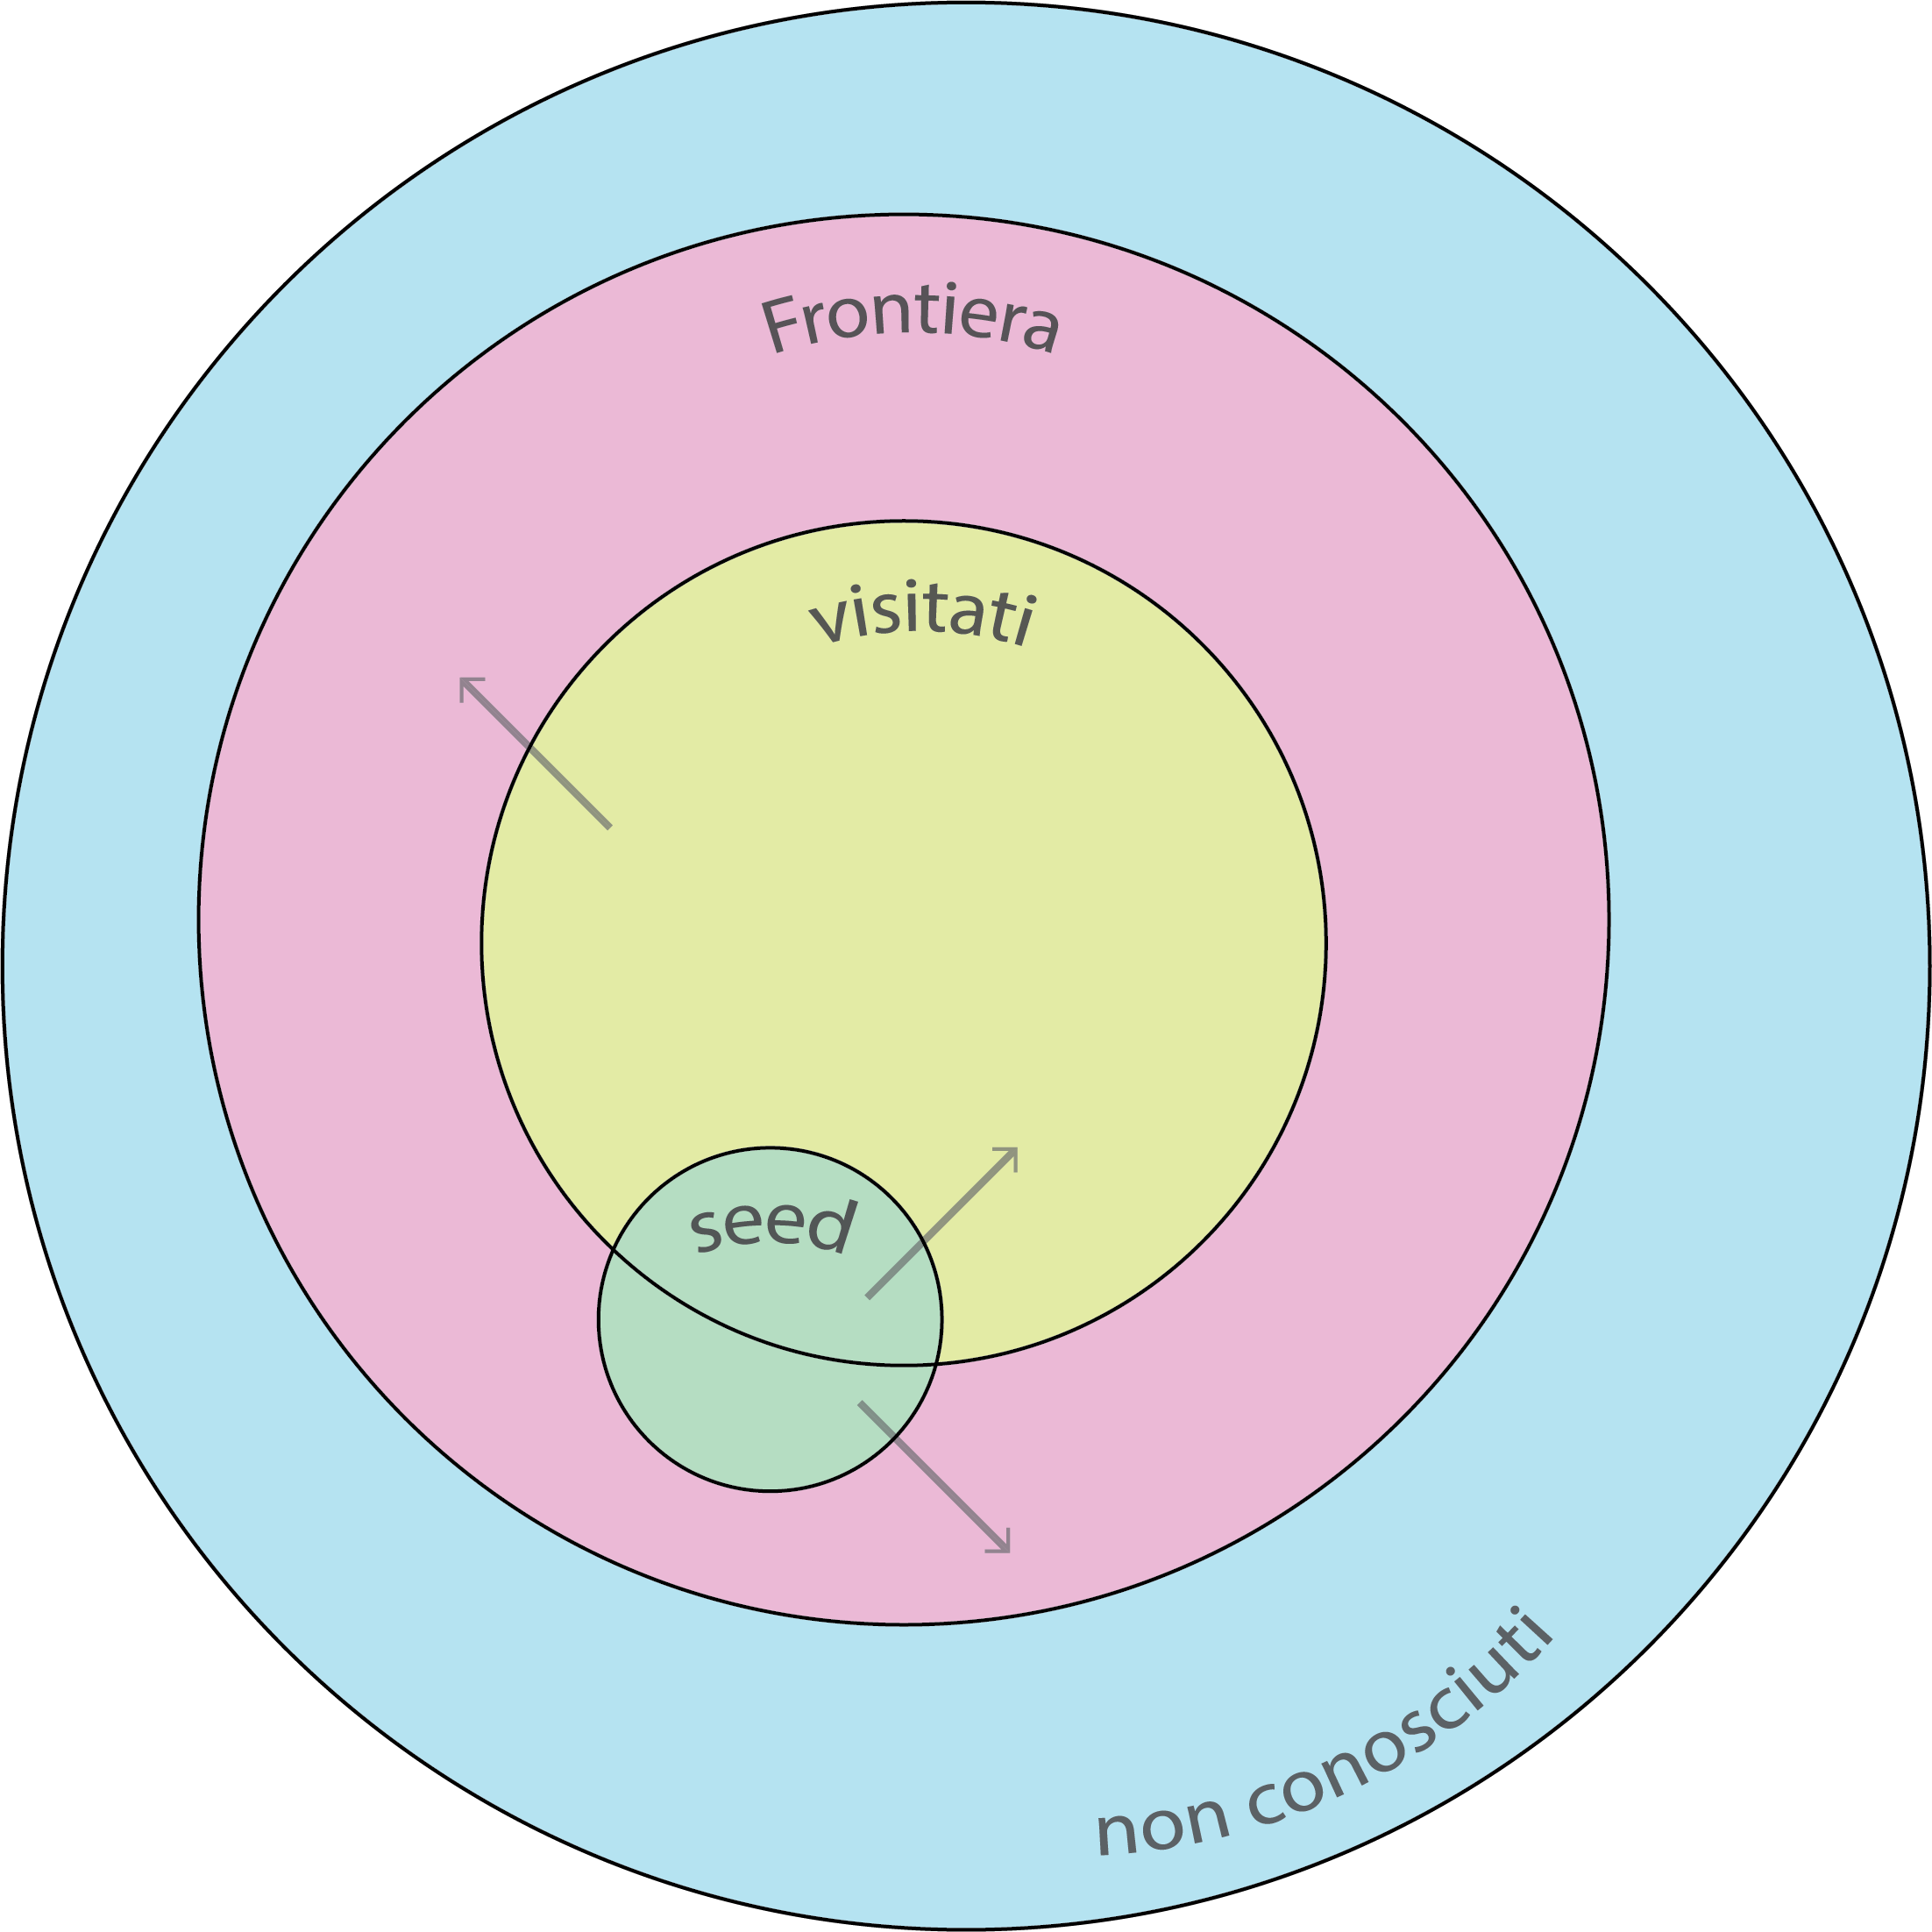
\includegraphics[width=70mm]{image/seed_frontiera_universo.png}
	\caption{seme, frontiera e universo}
	\label{fig:seme_front_universe}
\end{figure}

\begin{itemize}
    \item V: insieme dei visitati
    \item F: frontiera - URL conosciuto (perchè sono nel seed o sono raggiungibili da un nodo già visitato) ma non sono ancora stati visitati
    \item U: unknown
\end{itemize}
Nello stato iniziale F = S e V = 0

Dobbiamo prestare attenzione alla scelta del seed, una cattiva scelta di questo potrebbe portare a non visitare molti nodi nel grafo (il web ha una struttura "bowtie" il che rende non raggiungibile un insieme di nodi - specie con un bad seed, fortunatamente il web è composto da una componente connessa che include il 60-70\% dei nodi)
Dobbiamo prestare attenzione anche alla gestione della frontiera, essa occupa molto spazio in memoria e nel momento in cui arriva un nuovo URL devo sapere velocemente se sia già presente o meno).

Il crawling si differenzia da una semplice visita di un grafo per:
\begin{itemize}
    \item non sappiamo a priori quanto sarà grande il nostro grafo
    \item nella visita non abbiamo problemi di politeness
    \item identificatori delle pagine possono essere stringhe irregolari
\end{itemize}

\section{Mercator sieve}
\label{sec:Mercator sieve}
Il crivello è la struttura dati alla base del crawler: accetta in ingresso URL potenzialmente da visitare e fornisce come output URL pronti per la visita. E' necessario non emettere URL duplicati e rispettare l'ordine di arrivo di essi nel crivello. Per fare ciò il sieve unisce le caratteristiche di un dizionario con quelle di una coda con priorità - esso rappresenta la frontiera, il set dei visitati e la coda di visita. Il sieve di Mercator originale restituisce gli URL in ordine FIFO implementando una visita in ampiezza.

Il crivello di Mercator implementa un meccanismo di \textit{graceful degradation}, esso occupa uno spazio fisso in RAM scaricando parte del carico su disco. All'aumentare del carico il sistema andrà più lento senza causare l'esaurimento della memoria centrale. 

Il crivello è \textit{probabilistico}: rappresentiamo un URL con una firma tramite una buona funzione di hash. 

Il crivello utilizza 3 vettori: il vettore S in memoria centrale, il vettore Z su disco e il vettore A su disco.
\begin{itemize}
    \item il vettore S contiene tutte le firme degli URL che arrivano al crivello
    \item il vettore Z contiene tutte gli URL mai visitati ordinati
    \item il vettore A contiene tutti gli URL che arrivano al crivello, parallelamente al vettore S
\end{itemize}

Quando un URL arriva al crivello ne viene calcolata la firma, essa viene inserita all'interno del vettore S. Parallelamente l'URL è inserito nel vettore A. 
Il processo diventa interessante quando S e A sono pieni. Il vettore S viene ordinato indirettamente e stabilmente utilizzando la firma degli URL come chiave. A questo punto possiamo eliminare i duplicati da S marcando solo i primi. Effettuiamo un merge tra Z e S in un file Z'. \textit{Possiamo farlo in tempo lineare dato che sia S che Z sono ordinati}. Grazie a ciò possiamo marcare gli elementi che sono in S e che non risultano in Z, cioè firme di URL mai visitati. Infine possiamo scandire S e A in parallelo, per ogni firma di URL marcata in S ottengo URL corrispondente in A e lo inserisco nella coda di visita. S e A vengono svuotati e Z è sostituito con Z'.

\section{Gestire la politeness}
\label{sec:gestire la politeness}
Non si dovrebbe eccedere nella quantità di tempo dedicato allo scaricamento da uno stesso host. 

\begin{enumerate}
    \item \textbf{delay tra richieste consecutive} - attendo un tot di tempo tra la fine di una richiesta e l'inizio di un'altra
    \item \textbf{alternare fasi di accesso con fasi di attesa} - il crawler ha un tempo di accesso nel quale fa richieste all'host e un tempo in cui attende. Questo conviene: se un sito è veloce otterrò molti URL nell'arco di tempo, se un sito è più lento ne otterrò meno, in ogni caso rispettando la politeness. Inoltre questo permette di sfruttare una caratteristica di HTTP 1.1 che rende possibile effettuare più richieste attraverso la stessa connessione TCP.
\end{enumerate}

Per rispettare la politeness si rende necessario riorganizzare la frontiera: rispettare l'ordine della coda di visita potrebbe portare molti thread ad essere in stato di attesa (rischio di fermare tanti threads quando magari ci sono URL in un altro punto della frontiera che possono essere visitati)

\section{Coda degli host e concorrenza}
\label{sec:coda degli host e concorrenza}
Nell'attività di crawling è ovviamente conveniente avere molti thread che scaricano URL da diversi siti in contemporanea, questi thread saranno spesso in attesa I/O. Le pagine scaricate sono analizzate da un piccolo numero di thread (che eseguono operazione CPU bound). Considerando questo e considerando la politeness vogliamo evitare che due thread accedano allo stesso sito.

Per risolvere il problema della concorrenza e della politeness possiamo riorganizzare la frontiera - cioè gli URL emessi dal crivello. Per ogni host la priorità diventa il primo istante di tempo in cui è possibile scaricare dati da esso rispettando la politeness. La frontiera viene riorganizzata come una \textbf{coda con priorità}. Per ogni host manteniamo una coda (FIFO se BFS). Quando gli URL sono emessi dal crivello vengono indirizzati verso l'host a cui appartengono. 

Ogni thread prende l'host in cima alla coda (quella con l'istante disponibile minore), scarica dati da esso e poi lo mette in fondo alla coda aggiornando la sua priorità. Questo risolve anche il problema di concorrenza in quanto l'elemento della coda è come un token e rappresenta l'autorizzazione a scaricare da un dato sito. Un solo thread alla volta può avere il token di uno specifico sito.

Creare una coda con priorità potrebbe essere una buona idea anche per l'indirizzo IP.

\section{Near-duplicates e dizionari approssimati}
\label{Near-duplicates e dizionari approssimati}
Durante l'attività di crawling, è comune trovare pagine che sono quasi uguali (ci sono alcune pagine con URL diversi ma con stesso contenuto).Un modo semplice di risolvere questo problema in memoria centrale è calcolare una forma normalizzata del testo di una pagina (e.g. eliminare markup e date) e memorizzarli in un dizionario approssimativo (e.g. Filtri di Bloom). Metodi più sofisticati possono essere applicati offline.

\section{Filtri di Bloom}
\label{Filtri di Bloom}
Struttura dati probabilistica che rappresenta un insieme di elementi. Permette di aggiungere elementi e chiedere se un elemento appartiene o meno all'insieme, con il rischio di un falso positivo.

Partiamo da un universo U di elementi, definiamo un \textbf{vettore A di m bit} e \textbf{d funzioni di hash} h\textsubscript{0}, h\textsubscript{1},..., h\textsubscript{d-1} con h: U$\xrightarrow{}$ [0...m] 

\noindent Poniamo di voler aggiungere l'elemento x $\in$ U nel filtro, calcoliamo h\textsubscript{0}(x), h\textsubscript{1}(x),..., h\textsubscript{d-1}(x). Settiamo a 1 tutti i bit A[h\textsubscript{k}(x)] con 0$\leq{}$k$\leq{}$d. 
Intuitivamente ogni volta che aggiungiamo un elemento al filtro la probabilità che quell'elemento ci sia è divisa tra le d funzioni di hash, queste funzione di hash sono richieste quando c'è bisogno di sapere se un elemento è nel filtro o meno. 

\noindent Per sapere se un elemento è nel filtro, dato l'elemento  x $\in$ U, calcoliamo h\textsubscript{0}(x), h\textsubscript{1}(x),..., h\textsubscript{d-1}(x) e verifichiamo che tutti i bit A[h\textsubscript{k}(x)] siano = 1. E' possibile che qualcuno di questi bit sia stato settato = 1 aggiungendo un altro elemento y$\not=$x, per questo è possibile ottenere \textbf{falsi positivi}.

Il nome filtro in effetti deriva dall'idea che la struttura dovrebbe venire usata per filtrare le richieste a una struttura dati soggiacente più lenta. Se si prevede che la maggior parte delle richieste avrà risposta negativa, un filtro di Bloom può ridurre significativamente gli accessi alla struttura soggiacente. 

Stimiamo ora la probabilità di un falso positivo

\clearpage

\section{Crawling distribuito}
\label{Crawling distribuito}
Invece di effettuare un'attività di crawling su una macchina singola, impiego una farm. Per coordinare un insieme A di agenti indipendenti che effettuano attività di crawling è necessario assegnare in qualche modo ciascun URL ad uno specifico agente (è meglio distribuire host e non URL). 

Chiamiamo $\delta$\textsubscript{A}(u): U$\xrightarrow{}$A la funzione che dato un URL mi restituisce l'agente che se ne occupa. La funzione deve soddisfare due proprietà:

\begin{enumerate}
    \item \textit{Bilanciamento}
     \begin{equation}
      |\delta\textsubscript{A}\textsuperscript{-1}(a)| = |U|/|A|
     \end{equation}
     Se l'insieme di agenti A è statico basta fissare una funzione di hash h(u)mod$|$A$|$. Ma un caso più interessante è quello in cui l'insieme A degli agenti è dinamico e in questo caso la funzione $\delta$\textsubscript{A}() deve rispettare anche la proprietà di controvarianza
     
    \item \textit{Controvarianza}
    \begin{equation}
         A\subseteq B, 
         \delta\textsubscript{B}\textsuperscript{-1}(agente)\subseteq \delta\textsubscript{A}\textsuperscript{-1}(agente) 
    \end{equation}
    Questo mi dice che aggiungendo agenti, gli URL che appartenevano ad un agente di A sono un sottoinsieme di quelli che gli appartengo ora. Aumentando il numero di agenti, l'insieme di URL che erano associati ad un agente diminuisce. In particolare, se aggiungiamo un nuovo agente, gli agenti preesistenti non riceveranno nuovi URL.
\end{enumerate}
    
Ci sono tre modi di implementare questa idea

\subsection{Permutazioni aleatorie}
\label{Permutazioni aleatorie}    
Assumiamo esista un insieme P di agenti, e un sottoinsieme A$\subseteq$P di agenti attivi. Per semplicità possiamo assumere che P è formato dai primi $|$P$|$ numeri naturali, ma importa solo che P sia ordinabile. Fissiamo un generatore di numeri pseudocasuali, prendo un URL u nel calcolo h(u) e con il risultato inizializzo il generatore di numeri pseudocasuali, quest'ultimo lo uso per ottenere una permutazione aleatoria di P. L'agente che viene assegnato è il primo agente della permutazione di P che sta anche in A. 

Le permutazione sono generate uniformemente e in modo aleatorio, questo approssimativamente dà la stessa frazioni di URL a ciascuno agente. La controvarianza è garantita dal fatto che se consideriamo A$\subseteq${B} le uniche variazioni di assegnazione consistono nello spostamento di URL verso elementi di B$\setminus${A}

Dato che la permutazione è generata tramite un generatore comune a tutti gli agenti e usa lo stesso seme (u) tutti gli agenti calcolano lo stesso ordine di preferenza, non c'è esigenza che gli agenti comunichino tra loro.

La permutazione è generata in tempo lineare con la tecnica \textit{Fisher-Yates shuffle}.
Si noti che in realtà non è necessario generare l'intera permutazione: non appena competiamo l'iterazione i, se troviamo in posizione i un elemento di A possiamo fermarci. 

Le permutazione aleatorie sono un metodo semplice ma funziona solo se l'insieme di agente è ordinabile e non è sempre così. 

\subsection{Min-hashing}
\label{min-hashing} 
Il secondo approccio non richiede che ci sia un universo predeterminato ed ordinato.
Fissiamo una funzione di h(-,-) con argomenti un URL e un agente. L'agente a$\in$A responsabile dell'URL è quello che realizza il minimo tra tutti i valori h(u,a),  $\forall$ a$\in$A.
Assumendo che h sia aleatoria il bilanciamento è banale, ma lo è anche la controvarianza: aggiungendo agenti, gli unici URL che si spostano vanno nell'insieme B$\setminus${A}, dove h(b,u) $<$ h(a,u).

Questo metodo richiede tempo di calcolo proporzionale ad A, e spazio costante(basta tener traccia dei minimi)

\subsection{Hashing coerente}
\label{Hashing coerente} 
Consideriamo una circonferenza di lunghezza unitaria e una funzione di hash random che mappa gli URL in [0,...,1] (quindi sulla circonferenza). Fissiamo anche un generatore di numeri pseudocasuali. 
Per ogni agente a$\in$A, usiamo a per inizializzare il generatore e generare C posizioni random sulla circonferenza. Per trovare l'agente responsabile dell'URL u partiamo dalla posizione h(u) sulla circonferenza e procediamo in senso orario fino a che non troviamo una replica di un agente, questo sarà l'agente incaricato dell'URL u. 

La posizione delle repliche è deterministica: partendo dallo stesso generatore e inizializzandolo con una funzione di hash sul nome dell'agente, tutti gli agenti costruiscono la stessa circonferenza rendendo non necessaria la comunicazione tra agenti. 

La funzione è controvariante: quando aggiungo un nuovo agente l'unico effetto è quello di spezzare tramite nuove repliche i segmenti preesistenti sulla circonferenza: una parte resta sul vecchio agente e una parte va sul nuovo.
La questione più delicata è il bilanciamento: se avessimo solo due repliche una per agente la funzione sarebbe molto squilibrata. La soluzione sta nel numero di repliche: se C è scelto sufficientemente grande i segmenti risultano così piccoli da poter dimostrare che la funzione è bilanciata con alta probabilità. 

La struttura può essere realizzata in maniera interamente discreta memorizzando interi che rappresentano le posizioni delle repliche in un dizionario ordinato (e.g. albero binario bilanciato).
Questo richiede uno spazio lineare in $|$A$|$ e tempo logaritmico in $|$A$|$

\subsection{Considerazioni generali}
\label{Considerazioni generali} 

\begin{itemize}
    \item Abbiamo funzioni deterministiche che trattiamo come aleatorie, non possiamo fare a meno del determinismo se no ogni agente otterrebbe risultati diversi
    \item Tutti i metodi hanno una catena di responsabilità - cioè un modo per vedere chi sarebbe il destinatario dell'URL. 
    \item Min-hashing e hashing coerente possono presentare collisioni (2 minimi o 2 repliche coincidono). Disambiguiamo deterministicamente, ad esempio con ordine alfabetico.
\end{itemize}

\chapter{Indicizzazione}
\label{cap:indicizzazione}
Parte di un motore di ricerca in cui si prendono le informazioni scaricate e le si rendono in una forma in cui è possibile rispondere alle interrogazioni. 
Possiamo paragonare questo alla costruzione di un indice in un libro: abbiamo una selezione di parole e ci dice a che pagine trovarle, nel motore di ricerca abbiamo una mappa di keyword in alcuni documenti. 
Una volta era più importante la \textit{recall}: quantità di documenti restituiti per ogni richiesta. Col passare del tempo il numero di risposte è aumentato e si sposta l'attenzione alla \textit{precision}: importa la precisione dei documenti restituiti.


\begin{enumerate}
    \item \textbf{tokenizzazione-segmentation}
    Fase in cui si trasforma una stringa di caratteri in un token, che poi sarà il termine dell'inverted index.
    \item \textbf{normalizzazione}
    Dobbiamo effettuare delle scelte riguardo ai termini da tokenizzare: downcasing (togliere le lettere maiuscole, Papa = papa), critical removal (rimuovere accenti), stemming (troncatura, rimuovere le possibili variazioni di una lingua)
\end{enumerate}
In generale oggi si spinge per una normalizzazione meno spinta.

La struttura dati che permette l'indicizzazione è un inverted index, esso ci ridà l'elenco dei documenti in cui compare il termine cercato, chiamato \textit{posting list} o \textit{lista di affissioni}.

\begin{itemize}
    \item stopwords: temine che indica le parole che compaiono spesso (congiunzione, and, or), indicizzarle tutte fa si che la struttura sia molto grande ma possono tornare utili per le query frasali
    \item hapax legomenon: parola che compare una volta sola nella collezione. Una volta non venivano indicizzate, ora servono per identificare in modo unico certi documenti.
\end{itemize}

Vogliamo passare da una lista di documenti ad una struttura dati che data una parola restituisca i documenti in cui essa è presente. Leggiamo i documenti, mano a mano che compaiono termini li numeriamo in modo crescente. Teniamo traccia, per ogni documento, della codifica numerica del termine e del documento in questione.
Una volta ottenuta una lista di duple $<$termine,doc$>$ ordiniamo stabilmente e indirettamente con chiave il numero del termine. Otterremo così una lista ordinata nella quale abbiamo tutti i documenti in cui compare il termine 0, poi tutti i documenti in cui compare il termine 1 e così via.
Si può notare che il numero di chiavi è molto inferiore rispetto al numero di elementi da ordinare (molti termini sono ripetuti). Per questo motivo è utile usare come algoritmo di ordinamento il \textbf{count sort}, esso infatti è lineare nel numero di chiavi.\medskip

Nell'indicizzazione posso tenere traccia anche di quante volte il termine appare nel documento (conteggio) e in che posizioni all'interno di esso.\medskip

Grado di precisione:
\begin{itemize}
    \item motore booleano - senza conteggi e posizione ci dice solo se il token c'è nel documento
    \item motore senza posizione - mi da un'idea approssimativa di quanto il termine è importante nel documento tramite il conteggio
    \item posso tenere traccia di tutte e tre le informazioni
\end{itemize}

Alla fine ottengo l'indice dei termini, cioè un insieme di liste di affissioni una per ogni termine.
Essendo la lista di tuple molto grande, non è possibile ordinarla tutta insieme in una volta sola, ne leggiamo una parte e la ordiniamo, ne leggiamo un'altra e la ordiniamo. 
Questo comporta il problema alla fine di unire le varie parti ordinate in un unico grande elenco di liste di affissioni. 

Abbiamo S0, S1, S2 segmenti che contengono liste di affissioni diverse ma in ordine lessicografico - l'idea è di creare una algoritmo che permetta una fusione degli indici passando una volta sola su tutti i dati.

\section{Fusione multiway}
\label{fusionemultiway}
Abbiamo tre segmenti S0, S1, S2 con un puntatore al primo termine e consideriamo una coda con priorità. Inserisco i tre segmenti nella coda con priorità l'ordine alfabetico del primo termine del segmento.
A questo punto considero il termine indicato dal segmento in cima alla coda e lo metto da parte, dopo aver fatto questo aggiorno la coda.

Questo algoritmo sfrutta il fatto che i termini sono ordinati alfabeticamente, questo consente di scandire ciascuno segmento una volta sola e in tempo lineare. Altrimenti dovrei fare molte seek su tutti gli indici, operazione molto onerosa.
Teniamo in memoria i termini che stiamo scandendo, il resto sono tenuti su disco.
\clearpage

\chapter{Codici istantanei}
\label{cap:codiciistantanei}
Il problema della grandezza dell'indice ha creato problemi di compressione di esso, non solo per renderlo più piccolo ma anche più veloce.
Generalmente memorizziamo tre tipi di informazioni in un indice:
\begin{enumerate}
    \item \textbf{documenti} - sequenze crescenti 
    \item \textbf{conteggi} - solitamente numeri piccoli
    \item \textbf{posizioni} - numeri crescenti e piccoli 
\end{enumerate}

I codici istantanei sono usati per memorizzare numeri piccoli con pochi bit e numeri grandi con tanti bit. 
Un codice è un insieme $ C \subseteq 2^* $, cioè un insieme di parole binarie. Definiamo l'ordinamento per prefissi $ x \preceq y \iff \exists z \: y = xz $. In un ordine parziale due elementi x e y sono inconfrontabili se nessuno dei due è minore o uguale all'altro.

Un codice è \textit{istantaneo} o \textit{privo  di prefissi} se ogni coppia di parole distinte del codice è inconfrontabile. Ad esempio il codice {0,1} è istantaneo, il codice {0,01,1} non lo è. Di fronte alla stringa 001 nel primo caso sono sicura che sia 0-0-1 mentre nel secondo caso può essere 0-01 o 0-0-1.

Un codice è \textit{completo} se ogni parola $ w \subseteq 2^* $ è confrontabile con qualche parola del codice. Quando un codice istantaneo è completo è impossibile aggiungere una parola senza violare l'istantaneità.

I codici istantanei comprimono in maniera ottima rispetto alle loro distribuzioni intese.

\section{Disuguaglianza di Kraft-McMillan}
\label{Disuguaglianza di Kraft-McMillan}
\clearpage

\section{Codici istantanei per interi}
\label{Codici istantanei per interi}
Partiamo dal definire i codici binari minimali

\begin{figure}[h]
	\centering
	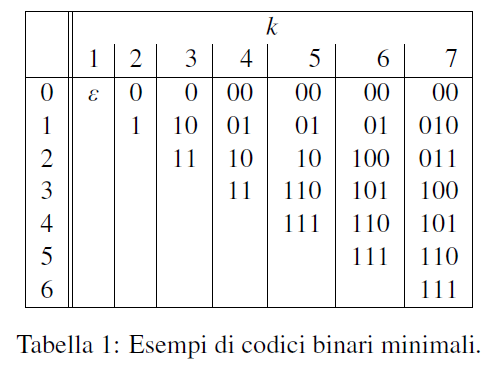
\includegraphics[width=80mm]{image/cod_minimali.png}
	\label{fig:cod_minimali}
\end{figure}

\subsection{Codice unario}
\label{codiceunario} 
Il codice unario rappresenta il numero x tramite x zeri seguiti da un uno. La lunghezza della parola del codice per x è quindi x+1. Il codice è banalmente istantaneo e completo. Le prime parole del codice sono 1,01,001,0001
\vspace{50mm}

\subsection{Codice Elias $ \gamma $ }
\label{codiceeliasgamma} 
Il numero x è rappresentato scrivendone la lunghezza in unario seguita dalla rappresentazione binaria ridotta di x (privata del bit più significativo). Il fatto che il codice sia istantaneo e completo si ottiene dal fatto che lo è il codice unario. La lunghezza della parola di codice per x è 2logx.
\vspace{50mm}

\subsection{Codice Elias $ \delta $ }
\label{codiceeliasdelta} 
Descrive il numero x scrivendone la lunghezza in Elias $\gamma$ seguita dalla rappresentazione in binario ridotta di x. Il fatto che il codice sia istantaneo lo ottengo dal fatto che lo è Elias $\gamma$. La lunghezza della parola di codice per x è logx + 2log(logx).
Elias $\delta$ risulta più impegnativo nei numeri piccoli, arrivati a circa 30 osserviamo che diventa più impegnativo Elias $\gamma$.
\vspace{50mm}

\subsection{Codice di Golomb di modulo b}
\label{codicegolomb} 
Descrive x scrivendone il quoziente x/b in unario, seguito dal resto in binario minimale. La lunghezza della parola di codice per x è x/b + 1 + log(b).
\vspace{40mm}

\subsection{Codice allineati a byte}
\label{codiciallineati} 
L'idea è che ogni parola è formata da un numero variabile di blocchi di k bit (8 per il byte). Il primo bit, detto di \textit{continuazione}, non fa parte dell'intero codificato e se è diverso da zero, indica che il codice non termina in quel blocco.
Ogni intero è diviso in blocchi di k-1 bit, tutti col bit di continuazione uguale a 1 tranne l'ultimo. Se x $\in$ [0...128] mi basta un blocco solo per la rappresentazione, se x è più grande mi servono più blocchi. Ho che il numero di blocchetti di k bit che mi servono per rappresentare x in binario sono $logx/k-1$, ognuna di queste unità costa k bit quindi $k* logx/k-1$ è il costo della parola del codice per x. Questo tipo di codice è istantaneo ma non completo.
\vspace{50mm}

\section{Codifiche alternative}
\label{Codifichealternative}

\subsection{Codifica interpolativa}
\label{codifica interpolativa} 
Una codifica non istantanea con risultati eccellenti. Abbiamo n\textsubscript{0}, n\textsubscript{1},..., n\textsubscript{s-1}$\in$[0...b]. Codifico il numero centrale n\textsubscript{s/2} con il suo codice binario minimale calcolato a seconda dell'intervallo [0...b]. Divido la sequenza in due intervalli $[0... x\textsubscript{s/2})$ e $[x\textsubscript{s/2 + 1}... b)$ e ripeto ricorsivamente il passaggio iniziale.

Un fatto interessante è che se avessi un intervallo [3...4] esso conterrebbe un solo intero, questo comporta che il codice binario minimale associato è la stringa vuota, senza consumo di bit. Un altro fatto è che la compressione non dipende dal distribuzione dei dati. In ultimo la decodifica di questo codice risulta scomoda perché devo decifrare tutto. 

\subsection{PFORDELTA}
\label{pfordelta}
Codifica per sequenze di numeri piccoli, tiene conto del fatto che uno dei costi fondamentali nell'elaborazione dei dati sono le scelte imprevedibili (Ogni CPU ha un'unità che predice eventi, la scelta prevista impiega molto molto meno tempo rispetto alla scelta sbagliata), i codici visti finora mettono a dura prova il predittore.

Si sceglie una dimensione di blocco B, x\textsubscript{0}, x\textsubscript{1},..., x\textsubscript{B-1}, e si trova una \textit{w} tale per cui il 90\% degli x\textsubscript{i} $<2^w$. A questo punto viene scritto un vettore B di interi di \textit{w} bit che descrive il 90\% dei dati, il restante 10\% è scritto separatamente in un altro vettore.
Nel primo vettore in corrispondenza di numeri che rappresentano eccezioni viene messa una sequenza di bit tutti a 1, in fase di decodifica del blocco quando incontro tutti i bit a 1 faccio un salto al vettore delle eccezioni.

Nel 90\% dei casi il predittore tira dritto senza effettuare controlli. Il principale svantaggio e che decodifico a blocchi, devo leggere tutto il blocco ogni volta.


\section{Codifiche per gli indici}
\label{Codifichepergliindici}
Nella scelta dei codici istantanei da utilizzare per la compressione di un indice è fondamentale la conoscenza della distribuzione degli interi da comprimere. In alcuni casi è possibile creare un modello statistico che spiega la distribuzione empirica riscontrata.

\begin{itemize}
    \item Per quanto riguarda i \textbf{conteggi}, la presenza di hapax legomena rende Elias $\gamma$ quello più usato.
            
    \item Per quanto riguarda le \textbf{posizioni} non esistono modelli predittivi adeguati per la rappresentazione, l'indice delle posizioni occupa il 90\% dell'indice. Utilizziamo un codice con buone prestazioni come il delta.
    
    \item La questione dei \textbf{documenti} associati ad ogni termine è più complessa. L'elenco dei puntatori documentali (documenti dei termini) è salvato a gap. Invece di salvare D\textsubscript{0}, D\textsubscript{1},..,D\textsubscript{n} salviamo D\textsubscript{0}, D\textsubscript{1}-D\textsubscript{0}, D\textsubscript{2}-D\textsubscript{1}...
    
    Il \textbf{modello Bernoulliano} di distribuzione prevede che un termine con frequenza \textit{f} compaia in una collezione di N documenti con probabilità p = f/N (casi favorevoli/casi possibili) in ogni documento indipendentemente (l'assunzione di indipendenza non è vera, pagine sugli stessi siti avranno argomenti comuni, ma è comoda per semplificare la situazione). Immaginiamo un vettore A, se A[i] = x nel documento sarà presente il termine, altrimenti non è presente. La probabilità di un buco, gap (e.g di lunghezza = 3) è (1-p)(1-p)(1-p)p. Il numero di (1-p) è la dimensione del mio gap, cioè i documenti dove il termine non compare. Un buco è lungo $(1-p)^k*p$ cioè una distribuzione geometrica.
    Abbiamo notato come il codice di Golomb abbia una distribuzione esponenziale negativa: si tratta quindi di trovare il modulo adatto a \textit{p}, è stato calcolato che il codice ottimo per una geometrica di ragione \textit{p} è un Golomb di modulo:

    \begin{equation}
        b = \lceil{log(2-p)/log(1-p)}\rceil
    \end{equation}

    
\end{itemize}





\section{Salti}
\label{salti}
Non è possibile ottenere in un tempo costante un elemento arbitrario di una lista compressa a gap: è necessario decodificare tutti i precedenti. I salti sono molto utili nella risoluzione di query congiunte (sto cercando Britney Spears, trovo Britney solo al k-esimo documento - ha senso iniziare a cercare Spears a partire dal k-esimo documento).

La tecnica di base per ovviare a questo inconvieniente è quella di memorizzare, insieme alla lista di affissioni, una tabella di salto che memorizza un certo numero di posizioni e valori ad intervalli regolari (dato un quanto q, memorizza il valore degli elementi con indice iq e le loro posizioni).

Quando si vuole effettuare un salto, cioè quando si vuole trovare il minimo elemento maggiore o uguale a b, si cerca nella tabella il massimo elemento di posto iq che sia minore o uguale a b, e si comincia a decodificare la lista per cercare il minimo maggiorante di b.

\chapter{Gestione liste di termini}
\label{gestionelistetermini}

Il motore di ricerca dovrà tener traccia del mapping tra i termini e gli interi, la lista dei termini in un indice può essere molto ingombrante. La tecnica che vedremo permette, data una lista di stringhe, di restituire il numero ordinale di qualunque elemento della lista, ma di \textbf{non memorizzare la lista stessa} (l'occupazione sarà circa di 5 byte per stringa, indipendentemente dalla lunghezza).

\section{Information theoretic Lower bound}
\label{lowerbound}

\noindent Abbiamo U insieme di stringhe e X termini del motore di ricerca (X$\subseteq$U). Ci serve una $f: X\to2^b = \{0...2^{b-1}\}$ dove b è il numero di bit.

\noindent Abbiamo T insieme di termini da memorizzare, per memorizzarli abbiamo bisogno di $\lceil$ log\textsubscript{2}$|T|$ $\rceil$ bit, quindi abbiamo bisogno di una mappa da T$\to 2^{log|T|}$.

\bigbreak
In generale se abbiamo una classe C con k oggetti per definire un oggetto di C mi servono almeno $\lceil$ log\textsubscript{2}$k$ $\rceil$ bit. Questo ci dice che ogni volta che memorizzo qualcosa c'è un costo in bit inevitabile, un lower bound.

Per quanto riguarda il nostro caso noi non vogliamo saper distinguere l'insieme delle chiavi, altrimenti non saremmo in grado di abbattere il lower bound. 
\bigbreak
\noindent Conto quanti sono i possibili sottoinsiemi di U di cardinalità X
\begin{equation}
    \binom{|U|}{|X|}
\end{equation}

\noindent Il coefficiente binomiale sopra mi ridà il numero di combinazioni di $|U|$ chiavi prese $|X|$ alla volta, per descrivere uno di questi insiemi di chiavi avrò quindi bisogno di 
\begin{equation}
   log\binom{|U|}{|X|}
\end{equation}
\noindent Se X è abbastanza piccolo
\begin{equation}
   |X| << \sqrt{U} \longrightarrow \approx{|X|log\frac{|U|}{|X|} }
\end{equation}

\noindent Nel nostro caso abbiamo un insieme U molto grande e un insieme $|X|$ molto piccolo. Ne segue che anche l'approssimazione sopra sia molto grande ($log|U|$ è molto grande). 

Sarebbe un uso di memoria enorme, dobbiamo togliere il ITLB. 

\section{Tecnica}
\label{tecnica}
Vogliamo scrivere una funzione $x \rightarrow{2^b}$ usando $c|X|2^b$ bit.

\noindent Le funzioni che da $|X| \rightarrow{2^b}$ sono ${2^b}^{|X|}$, quindi per ITLB avrò bisogno di 
\begin{equation}
    log({2^b}^{|X|}) \approx |X|log(2^b) = b|X| bit
\end{equation}
Aggiungiamo poi una costante \textit{c} $\rightarrow$ $c|X|2^b$ bit
\bigbreak
Non vogliamo memorizzare le chiavi, solo gli output. Se $|X|$ = n, significa andare ad utilizzare solo nb: b bit per n output. Non usiamo le chiavi poiché esse possono essere tante e lunghe.
\bigbreak
Parto da due assunzioni:
\begin{enumerate}
    \item struttura statica - abbiamo le chiavi, viene ridato un valore e non possiamo cambiarlo.
    \item struttura funziona solo su x - se interrogo la struttura ed x non è presente non mi viene ridato un valore speciale (null o -1) mi viene ridato un valore random.
\end{enumerate}

\noindent Chiamiamo $|X|$ = n.

\noindent Scegliamo quindi di creare due funzioni di hash \textit{h}: U$\to$ cn e \textit{g}: U$\to$ cn, con cn spazio dei valori un po' più ampio della cardinalità di X (cn $> |X|$). Creo poi un vettore \textbf{w} con \textit{cn} variabili da b bit, per cui occupa \textit{cnb} bit (indipendente dalla dimensione delle chiavi)

\noindent Per ogni x$\in$X 
\begin{equation}
    w\textsubscript{h(x)} \oplus w\textsubscript{g(x)} = f(x)
\end{equation}
\bigbreak

\noindent A questo punto, ad esempio, se voglio sapere f(a) prendo $ w\textsubscript{h(a)} + w\textsubscript{g(a)}$. In generale posso quindi sapere la funzione per ogni stringa senza aver memorizzato la funzione stessa, usando il vettore \textbf{w}.

\bigbreak
\noindent Dovrò tenere in memoria h(x) e g(x) (parametri da 64 bit) e salvare da qualche parte il vettore w. Dobbiamo assicurarci solo che il sistema sia risolvibile, se non lo è sceglieremo altre due funzioni di hash, e che il numero di variabili non sia eccessivo (dovrò anche capire come dimensionare \textit{c})

\bigbreak
\noindent La struttura è statica perché cambiando un valore mi cambia tutto. In secondo luogo la struttura funziona solo su x perché nel caso prendessi un elemento non presente in X, calcolerei h(x) e g(x) che mi ridarebbero due variabili all'interno del vettore w. Farei poi una somma sulle variabili trovate che però sono variabili "random" che mi restituiscono un valore di funzione "random". Per questo motivo non ho un valore particolare quando x non si trova nell'insieme, mi viene restituito un numero casuale.

\bigbreak
\noindent \textbf{Come faccio a sapere se l'elemento x è nell'insieme o meno?}
Per ogni elemento x nell'insieme, calcoliamo h(x) e creiamo una tabella S che contiene tutte le firme di ogni termine. 

\begin{enumerate}
    \item Calcoliamo l'output di x, cioè f(x) che è un numero
    \item Recuperiamo S\textsubscript{f(x)}
    \item Se S\textsubscript{f(x)} = s(x) restituiamo f(x), altrimenti -1
\end{enumerate}
Si noti che se x$\in$X, f(x) è il suo rango in X, e quindi S\textsubscript{f(x)} conterrà per definizione s(x).

\bigbreak
\noindent \textbf{Come assicuro in un tempo ragionevole la presenza di un sistema risolvibile?}
\noindent Rappresento il sistema come un grafo non orientato tenendo conto del sistema di partenza, i nodi del grafo sono le variabili e gli archi le equazioni. 
\vspace{50mm}

\noindent Risolvere il sistema equivale a fare \textit{pealing} sul grafo, cioè pelare le foglie del grafo. Quando peliamo una foglia abbiamo tolto una variabile che sta in una sola equazione (le foglie hanno grado uno per definizione, quindi una sola equazione nella variabile). Mano a mano che pelo la variabile V\textsubscript{i}, V\textsubscript{i} non comparirà più nelle equazioni successive. 

Mano a mano che pelo creo uno stack di equazioni.
Una volta che ho finito le foglie rimango con un nodo solo, considero l'ultima foglia pelata e la relativa equazione tra di essa e l'unico nodo rimasto nel grafo. Assegno un valore all'unico nodo rimasto e risolvo l'equazione in modo tale da ottenere f(x) nota. Risalgo seguendo l'ordine di pealing, avrò sempre una variabile libera nelle equazioni che incontro poiché pelo foglie, assegniamo in maniera greedy i valori alle variabili.
\bigbreak
\noindent \textbf{Non posso risalire alla soluzione se il grafo è ciclico}. C'è una legge per la ciclicità: se il grafo ha \textit{cn} vertici e \textit{n} lati, se c è molto grande probabilmente il grafo è aciclico perchè ho molti più nodi che archi. La soglia che ci garantisce l'assenza di cicli è c$>$2.09, è un'approssimazione ma per noi va bene (facciamo un sistema usando un numero di variabili che è più del doppio del numero di equazioni). 

\noindent memorizzo la soluzione usando 2.09\textit{nb}, è peggio di \textit{bn} bit, ma siamo slegati da X.

\noindent Tutto questo si può fare con i k-hypergraphs che sono grafi normali con lati da k nodi. 
Nei 3-hypergraphs C=1.23, essi vengono usati con equazioni con 3 variabili e 3 funzioni di hash. 

\section{Rango su vettori di bit}
\label{rangosuvettoridibit}
Il rango considera  una posizione in un vettore e restituisce il numero di 1 precedenti a quella posizione (se mi serve una maschera di bit che contenga k 1, esso è il numero $2^{p}-1$)

\begin{enumerate}
    \item Un primo metodo per calcolare il numero di 1 prima di una posizione è il POP COUNT, esso conta il numero di bit diversi da 0 in una parola. Possiamo prendere il vettore e dividerlo in parole (ad esempio da 64bit) e facciamo pop count fino a che non arriviamo alla posizione di interesse.
    \item C'è anche un secondo metodo. Ho un vettore A che contiene molti zeri. Costruisco un vettore D in modo tale che D[i] = 1 quando l'elemento A[i]$\ne$ 0, D[i] = 0 quando A[i] = 0 (se ad esempio l'elemento di A è una parola da 64 bit, il vettore D è molto più piccolo). Costruisco il vettore A\textsuperscript{'} con i soli elementi non nulli in A.

    A questo punto vado nel vettore D, se D[i]=0 restituisco 0 mentre se D[i] = 1 ne calcolo il rango e ci indicizzo il vettore A\textsuperscript{'} che mi restituisce l'elemento di A $\ne$0
\end{enumerate}

\chapter{Risoluzione delle interrogazioni}
\label{risoluzionedelleinterrogazioni}
Processo che va dal bisogno dell'utente al motore di ricerca, un utente cerca t e vuole indietro la sua lista di affissioni S$\subseteq$D.
La risoluzione di un'interrogazione dipende fondamentalmente da due fattori:
\begin{itemize}
    \item il linguaggio di interrogazione e la corrispondente semantica
    \item il tipo di dati contenuti nelle affissioni dell'indice
\end{itemize}
\noindent La semantica [[ ]] di un termine è data dalla lista di documenti in cui il termine compare. 
\bigbreak

    [[t]] lista di affissioni
    
    [[q1$\land$q2]] $\to$  [[q1]]$\cap$[[q2]]
    
    [[q1$\lor$q2]] $\to$  [[q1]]$\cup$[[q2]]
    
    $\neg$q $\to$ D/[[q]]
    
\bigbreak
\noindent Dobbiamo farlo in modo pigro perché non possiamo scaricare tutta la lista di q1 e poi tutta quella di q2 e fare intersezioni/unione verrebbe troppo lungo. Il modo pigro è leggere dalle lista in input solo i puntatori necessario ad emettere un certo prefisso dell'output. Questo permette di gestire in maniera efficace la \textit{terminazione anticipata}, tecnica con cui il calcolo della semantica viene arrestato sulla base di stime della qualità dei documenti già rinvenuti.

L'utente non sa che policy di trasformazione è stata scelta per i termini in fase di indicizzazione (stemming, eliminazione di lettere maiuscole), è importante quindi che quando viene eseguita una query essa passi per lo stesso tipo di trasformazione.

\begin{itemize}
    \item \textbf{OR} - Per fondere liste in tempo lineare è sufficiente una coda di priorità indiretta che contiene i puntatori alle liste, ordinate secondo il documento corrente. Con solo due liste posso restituire il minimo, quando ho più di due liste funziona allo stesso modo della fusione multiway. OR è lazy perché appena ho un documento pronto posso emetterlo senza aspettare lo scorrimento di tutte le liste.
        
    \item \textbf{NOT} - Ho una lista di documenti che soddisfano q e io voglio tutti gli altri. 
    e.g. leggo D\textsubscript{0} = 0 e non lo considero, leggo D\textsubscript{1} = 6, per rispondere alla query considero i documenti 1, 2, 3, 4, 5. Dovrebbe essere lazy perché emette risultati quando può, senza aspettare la fine della lista
    
    \item \textbf{AND} - Per quanto riguarda l'intersezione, sebbene in linea di principio il limite inferiore lineare non sia superabile, esistono diverse euristiche che permettono di accelerare la computazione nel caso l'indice fornisca la possibilità di effettuare \textit{salti} - vale a dire muoversi rapidamente fino a un documento dato. 
    
    In linea di principio, potremmo tenere conto tramite una coda con priorità indiretta del documento minimo corrente, ma tenere al tempo stesso traccia del massimo puntatore in una variabile. Quando coincidono, il puntatore sta nell'intersezione e può essere restituito (immediatamente dopo una lista viene fatta avanzare)
    \vspace{50mm}
    
    Il tempo richiesto è lineare nella dimensione di input, possiamo fare meglio di così. Per migliorare l'algoritmo l'idea è che avanzare in maniera miope le liste fino al massimo corrente \textit{m} finché non sono tutte allineate. Al primo disallineamento  si ricomincia ad allineare la prima lista. Quando si arriva ad allineare l'ultima lista, si ha un puntatore da restituire
    \vspace{50mm}
    
    Possiamo migliorare ulteriormente, non ci serve più una coda. Troviamo un match sulle prime due liste, quando lo troviamo cerchiamo un match con la terza lista in cui effettueremo un salto molto lungo. Una volta allineate le tre liste, avanzo le prime due e cerco di riallinearle, e poi procedo come prima.
    \vspace{50mm}
    
    Un ultimo miglioramento riguarda l'ordinare le liste in ordine di frequenza (se conosco la densità delle parole nei documenti, faccio prima intersezione tra parole che non sono molto dense). Se dovessi risolvere la query "Romeo e Giulietta", potrei trovare prima l'intersezione tra "Romeo" ed "e" ma essendo "e" è molto denso, cercare questa intersezione mi ridarebbe la lista di affissioni di "Romeo" (meno densa di "e"). Ordinando per frequenza la maggior parte degli avanzamenti verrà giocato dalle prime liste, che essendo quelle di minima frequenza genereranno pochi allineamenti. Le liste più frequenti subiranno pochi avanzamenti ma molto consistenti.
    
\end{itemize}
\bigbreak

Non voglio estrarre tutti i documenti, ne estraggo una parte e ad un certo punto smetto, \textbf{terminazione precoce}. Dovrei avere i documenti ordinati per validità ed importanza (ci sono documenti che finisco nel Google Hell e non vengono mai indicizzati avendo numeri molto grandi). Dopo che ho fatto crawling ordino la lista dando importanza a documenti di qualità. 
\bigbreak

\section{Query frasali}
\label{query frasali}
In generale quindi per rispondere alle query è necessario effettuare una ricerca booleana sui termini, una volta ottenuti i documenti che contengono i termini, controllo le posizioni per cercare i termini vicini. 
Abbiamo ad esempio cercato "Romeo e Giulietta", abbiamo trovato i documenti interessati e ora abbiamo un documento di posizioni.

\begin{itemize}
    \item \textit{Romeo} p\textsubscript{0}, p\textsubscript{1}, p\textsubscript{2},..
    \item \textit{e}  q\textsubscript{0}, q\textsubscript{1}, q\textsubscript{2},..
    \item \textit{Giulietta } r\textsubscript{0}, r\textsubscript{1}, r\textsubscript{2},..
\end{itemize}
\bigbreak
\noindent Devo quindi cercare la frase r\textsubscript{0} = q\textsubscript{0}+1 e q\textsubscript{0} = p\textsubscript{0}+1.
\noindent E' come intersezione, lo faccio come prima senza salti avanzando sequenzialmente. Devo rinumerare le liste:

\begin{itemize}
    \item \textit{Romeo} p\textsubscript{0}, p\textsubscript{1}, p\textsubscript{2},..
    \item \textit{e}  q\textsubscript{0}-1, q\textsubscript{1}-1, q\textsubscript{2}-1,..
    \item \textit{Giulietta } r\textsubscript{0}-2, r\textsubscript{1}-2, r\textsubscript{2}-2,..
\end{itemize}

\section{Distribuzione - segmentazione dell'indice}
\label{indici distribuiti}

Le dimensioni degli indici del web sono tali da rendere poco pratico l'accumulo dell'intero indice su una sola macchina. E' quindi necessario segmentare l'indice in sottoindici, detti \textit{segmenti}, le cui risposte verranno poi opportunamente
combinate. In linea di principio, un indice può essere partizionato tramite una funzione che assegna ad ogni affissione un segmento destinazione. Ad ogni segmento saranno associati i termini per i quali compare almeno un'affissione.
In pratica, però, è più comune scegliere un singolo criterio di partizionamento, \textit{documentale} o \textit{lessicale}.
\bigbreak

\noindent \textbf{Segmentazione lessicale:}
\noindent posso dividere in blocchi la collezione di termini usando un ordine lessicografico (A-L sul primo computer, M-Z sul secondo computer).In questo modo la lista di affissioni relativa ad un termine sarà interamente contenuta nel segmento relativo.

Nelle interrogazioni cambia che il server elabora la query e chiede i risultati ai PC, richiedendo che il server abbia un accesso molto veloce ad essi. Potrebbe essere anche comodo ordinare i termini all'interno dello stesso PC (i termini più richiesti in RAM, termini via di mezzo su SSD e termini rari su HDD)

\begin{itemize}
    \item + dividiamo il carico di lettura su più macchine
    \item - dobbiamo trasmettere i dati via rete che è molto più lento di una lettura dalla memoria, ci dev'essere un server sopra che risolve le query che non possono essere risolte da un pc singolo
\end{itemize}
\bigbreak
\noindent \textbf{Segmentazione documentale:}
\noindent posso dividere le liste di affissioni a blocchi (da 0 a 500.000 sul primo PC, da 500.001 a 1 mln sul secondo e così via), ci sarà un server che coordina tutto come nel caso sopra. In pratica tutte le affissioni relative ad un blocco vanno in un segmento e al segmento saranno associati i termini che compaiono nel blocco. Solitamente lo stesso termine comparirà in più segmenti (termini comuni come le congiunzioni), mentre gli hapax legomena compariranno esattamente in un solo segmento. 

\begin{itemize}
    \item + è scalabile: posso aggiungere una macchina semplicemente
    \item + il server deve solo concatenare i risultati, la risoluzione delle query booleane è affidati ai singoli server. 
\end{itemize}

Se ho le liste in ordine di qualità dei documenti i primi server saranno molto sotto pressione rispetto agli altri. Per ovviare possiamo avere molti server sui documenti iniziali e sempre meno nei documenti alla fine. 
\bigbreak
\noindent \textit{Adesso è usata la segmentazione documentale. Un'idea è usare la documentale su più macchina e usare la lessicale all'interno della stessa dividendo i termini in Ram, disco, SSD}
\bigbreak

La ricostruzione delle liste di affissioni a partire da una segmentazione lessicale è banale: individuo il segmento che contiene il termine e lo interrogo. La ricostruzione delle liste di affissioni a partire da una segmentazione documentale è più delicata: bisogna interrogare tutti i segmenti per sapere quali possiedono una lista di affissioni per il termine dato. Le liste vanno poi combinate.

In entrambi i precedenti casi può essere utile filtrare le richieste ai segmenti tramite dei filtri di Bloom, che possono rappresentare in maniera molto compatta l'insieme di termini presente in ogni segmento. 

\chapter{Ranking}
\label{cap:ranking}
Nella sua forma più generale, un sistema di information-retrieval è dato da una collezione di documenti D di dimensione N, un set di Q query e una funzione di ranking r: QxD $\rightarrow{R}$. Questa funzione assegna a ogni coppia documento-interrogazione un punteggio (numero reale). L'idea è che per ogni query, assegniamo ad ogni documento un punteggio: zero se il documento non è rilevante e un punteggio direttamente proporzionale alla rilevanza del documento. 

Quando fissiamo la query q, il sistema assegna un \textit{rank} ai documenti, ordinandoli per importanza; il rank è essenziale per restituire i documenti in ordine, specie in sistemi che contengono collezioni molto grandi (l'utente guarderà pochi risultati per ogni query, è bene restuitire quelli più pertinenti).

Ci sono due tipologie di ranking - \textbf{esogeno} (dipende da fattori esterni al contenuto del documento) ed \textbf{endogeno} (dipende dal contenuto del documento)

\section{Ranking endogeno}
\label{ranking endogeno}
I metodi di ranking endogeno utilizzano il contenuto di una pagina per assegnarle un punteggio.

\begin{itemize}
    \item \textbf{TF} (Term Frequency o conteggio): conto quante vole il termine compare nel documento
    
    Ma TF è molto soggetto a manipolazione (riempire pagine di keyword bianche su sfondo bianco), inoltre se un documento è molto lungo avrò un un alto TF ma non necessariamente un documento più valido. Nell'interrogazione come Romeo e Giulietta il metodo di conteggio valuterà in maniera positiva documenti contenenti un grande numero di "e" (stiamo valutando interrogazioni non booleane, solo con la presenza di termini dei documenti)
    
    \item \textbf{IDF} (Inverse Document Frequency): se abbiamo una query su più termini, IDF considera i termini più rilevanti in essa. Con più rilevanti intendiamo termini con frequenza minore che danno un'informazione maggiore.
    
    \item \textbf{TF/IDF}: è una combinazione delle due sopra. Esso normalizza il conteggio dividendole per il massimo conteggio all'interno del documento, o per la lunghezza del documento, e inoltre lo attenua moltiplicandolo per l'inverso della frequenza del termine. Essendo la divisione per la frequenza molto forte, spesso il conteggio è moltiplicato per il logaritmo del numero di documenti diviso per la frequenza.
    
    In formule, se \textit{c} è il conteggio di un termine \textit{t} nel documento \textit{d} di lunghezza \textit{l} e \textit{f} è la frequenza di \textit{t} nella collezione documentale il peso di \textit{t} nella valutazione di \textit{d} è:

    \begin{equation}
        \frac{c}{l} log \frac{N}{f}
    \end{equation}
    
    Torniamo all'esempio di Romeo e Giulietta, il temine "e" comparirà in quasi tutti i documenti, e verrà quindi pressoché ignorato dallo schema TF/IDF (N/f $\approx$ 1)

    \item \textbf{BM25}: l'idea è che il ranking di un documento è la probabilità che il documento sia rilevante per l'utente, data una query.
    
    \begin{figure}[h]
	\centering
	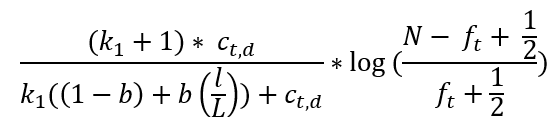
\includegraphics[width=90mm]{image/bm25_1.png}
	\label{fig:bm251}
    \end{figure}
    
    dove b e k\textsubscript{1} sono dei parametri liberi che devono essere tarati sulla collezione documentale, e L è la lunghezza media di un documento nella collezione. Si noti che la parte dentro al logaritmo è una versione di punteggio IDF. Vale la pena notare che la formula non è più lineare in \textit{c}, ma ha un limite asintotico k\textsubscript{1} + 1 (quindi un numero eccessivo di ripetizioni ha un'influenza bassa)
    
\end{itemize}

\section{Ranking esogeno}
\label{ranking esogeno}
Non si base sulle caratteristiche interne di una pagina, è un punteggio che viene ricavato dalle pagine che puntano quella per cui sto calcolando il rank. Quando si parla di ranking esogeno si fa riferimento alla struttura della rete. 
\clearpage

\chapter{Hyperball}
\label{cap:hyperball}
Affrontiamo un problema più generico della centralità $\rightarrow{}$ dato un grafo vogliamo calcolare la distribuzione delle distanze tra i vertici. Questo distribuzione esprime bene quanto sono vicini e quanto sono lontani i nodi di una rete e mi da un'idea globale della rete che tiene conto della struttura. 

Ci basiamo sul calcolare le sfere intorno ai nodi (sfera di raggio = 1 è l'outdegree, sfera di raggio = 2 sono i vicini a distanza 2 e così via). Prendo tutte le sfere a distanza t e le divido per la somma di tutte le loro cardinalità e ottengo distribuzione. 

Non possiamo mantenere tutto in memoria per cui procediamo con ordine: lo facciamo per tutte le sfere con raggio 0, poi per tutte quelle con raggio 1 e così via. 
\bigbreak
\noindent \textbf{Il problema è il calcolo delle sfere di dimensione t per ogni nodo}

\noindent Potremmo fare molto BFS, ma verrebbe molto dispendioso.
\bigbreak
\noindent Ragioniamo in termini di bolle, chiamiamo B\textsubscript{t}(x) la bolla di raggio t intorno a x (nodi con distanza al più t da x)

\begin{itemize}
    \item B\textsubscript{t}(0) = $\{x\}$ singoletto
    \item B\textsubscript{t+1}(x) = $\cup x\rightarrow{y} B\textsubscript{t}(y) \cup{\{x\}} $ la bolla di raggio t+1 di x è l'unione delle bolle di raggio t di tutti i vicini y di x, unito a x stesso
\end{itemize}

\noindent A noi interessa la dimensione della bolla e non come è fatta. 
\bigbreak

\noindent Prendiamo per esempio un grafo con sei vertici, rappresentiamo le bolle come maschere di bit (figura \ref{fig:hyperball1}).

Le frecce rappresentano le connessioni dei nodi nel grafo (il primo vertice ha come successori il secondo e il quarto ad esempio). I vettori al momento corrispondono alle bolle di raggio 0, in ogni bolla c'è solo il nodo stesso (nel disegno rappresentato dalla faccina sorridente).
\begin{figure}[h]
	\centering
	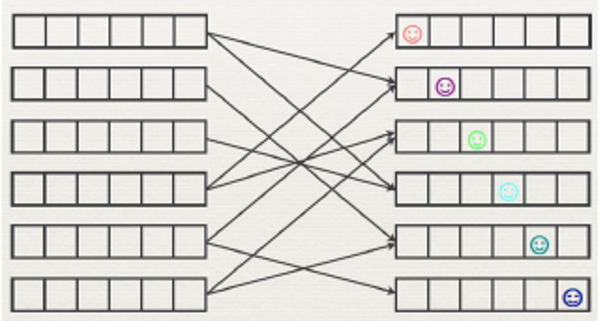
\includegraphics[width=105mm]{image/hyperball1.png}
	\caption{}
	\label{fig:hyperball1}
\end{figure}
Per trovare le bolle B\textsubscript{t+1} devo fare unione delle bolle B\textsubscript{t} più le bolle dei suoi successori, per farlo copio il vettore del primo vertice e prendo le maschere dei suoi successori, in questo il secondo e il quarto vertice (equivale a fare or).
\begin{figure}[h]
	\centering
	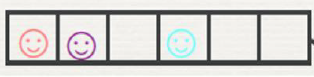
\includegraphics[width=50mm]{image/hyperball2.png}
	\label{fig:hyperball2}
\end{figure}

\begin{figure}[h]
	\centering
	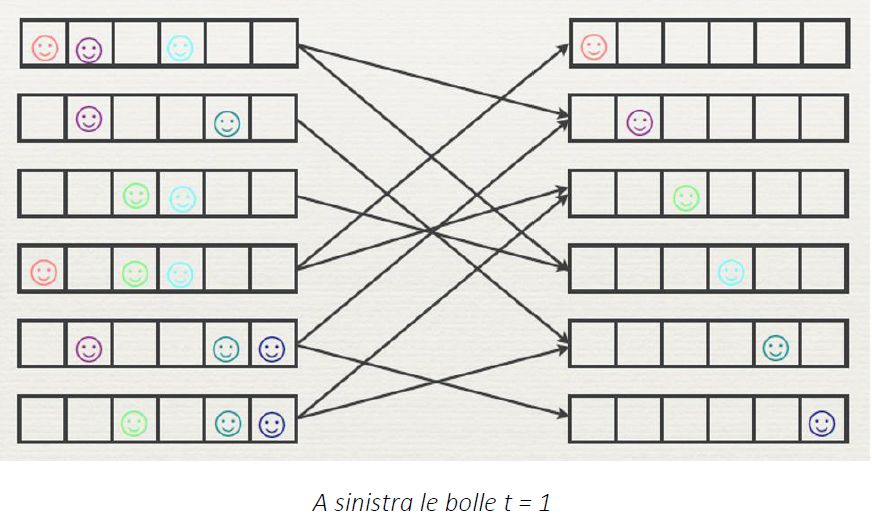
\includegraphics[width=110mm]{image/hyperball3.png}
	\label{fig:hyperball3}
\end{figure}
\clearpage
\begin{figure}[h]
	\centering
	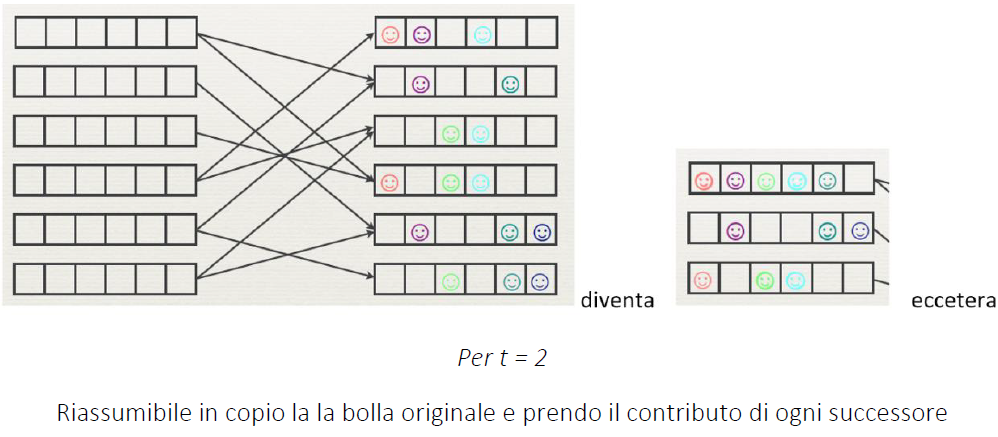
\includegraphics[width=140mm]{image/hyperball4.png}
	\label{fig:hyperball4}
\end{figure}

Ogni set occupa uno spazio lineare, complessivamente è usato uno spazio quadratico per cui si usa un \textbf{set approssimato}. Usiamo un counter probabilistico che rappresenta un set ma ci da solo informazioni sulla dimensione di esso. Ci va perfettamente bene perchè siamo interessati alla dimensione delle bolle e non ai nodi all'interno qualitativamente. 

\section{Hyperloglog counters}
\label{hyperlog}
La dimensione della struttura è loglog(n) dove n sono gli elementi da rappresentare. Un contatore normale è un dizionario che contiene chiave + conteggio, nel nostro caso le chiavi sono troppe. 

\noindent Idea: invece di memorizzare le chiavi, memorizziamo una feature statistica dell'insieme. Invece di ricordare cosa mette dentro, il counter ricorda un valore corrispondente estratto dalla chiave. 
\bigbreak
Si utilizza una funzione di hash che genera una stringa di bit. La caratteristica statistica che si intende memorizzare è il numero di \textbf{trailing zeros}, cioè il numero di zeri a DX della stringa. In particolare ricordiamo solo il numero massimo di trailing zero osservati fino a quel momento. Questo procedimento trasforma i nostri dati - che seguono una distribuzione non nota - in qualcosa, trailing zero, che so che segue una distribuzione geometrica. 
\bigbreak
Se mettiamo un elemento è probabile che sia una dispari (finisce con 1) quindi il massimo di TZ è 0. Se mettiamo almeno un paio di elementi, ci saranno numeri pari (finiscono con 0) con differente numero di zero a DX, quindi il massimo numero di zero sale. Siccome i valori sono generati in modo casuale sarà necessario fare molto inserimenti per avere un numero di zero a DX che aumenta il valore memorizzato nel contatore. In particolare è dimostrabile che sale con l'aumento esponenziale del numero di elementi inseriti $2^m$.

Il counter value (il numero memorizzati) è al più log(n); se estraggo n numeri a caso con elevata probabilità vedremo al più log(n) zeri a destra, cioè per avere più di log(n) zeri devo aver estratto casualmente più di n numeri. Per scrivere log(n) numero mi servono log(log(n)) bit.
\bigbreak
\textit{Se ho $10^9$ elementi, il numero massimo di 0 che vedrò con alta probabilità è 30 circa, $log(10^9) = 30$ è molto improbabile avere più di 30 zero se non estraiamo molto più di $10^9$ elementi. }
\bigbreak
E' stato dimostrato che esiste uno stimatore che è in grado di restituire il numero di elementi distinti che è stato inserito, che è approssimativamente $2^m$ (dove m è il valore massimo), quando chiedo size mi viene ridato $2^m$.
\bigbreak
Usiamo 6 bit per tracciare $2^64$ elementi: su 6 bit posso rappresentare $2^6 = 64$ trailing zero. Grazie a questo lo stimatore mi ridarà quindi $2^64$ elementi nel set.
\bigbreak
Oltre al contare serviva anche l'unione di due insiemi/contatori: per unire due contatori probabilistici ci basta prendere il massimo dei due: questo perchè è come se avessi messo tutti gli elementi dei due in un unico contatore, e visto che tiene memorizzato solo il massimo siamo a cavallo.
\bigbreak
\textbf{Allora ogni nodo ha un contatore che misura quanto è grande la bolla intorno a x di raggio t. All’inizio mettiamo x nel contatore di x per ogni contatore di ogni nodo. Per calcolare bolla di raggio successivo massimizziamo con i successori e unisco.}

\subsection{Aumentare affidabilità unendo più set (broadward)}
\label{broadward} 
E' una misurazione probabilistica dipendente dalla funzione di hash scelta, lo stimatore mi ridà $2^m$ \textit{ha una varianza molto alta}. Devo fare tante esecuzioni (sugli stessi elementi) con funzioni di hash diverse (cambiare funzione di hash mi cambia il numero di trailing zero) in modo da abbassare la varianza
\bigbreak
Per aumentare l'affidabilità, abbiamo bisogno di molti contatori e di prenderne la media armonica. Ogni set è rappresentato da una lista di registri a 6 bit, numero tipico ne prendo almeno 16*6bit = 96bit.
\bigbreak
Scegliendo un numero minore o maggiore di contatori avremo una stima più o meno precisa. O abbiamo tanta memoria e usiamo più registri (6 bit) per contatore quindi per vertice, o abbiamo un grafo enorme e ci teniamo 16 registri per contatore per stare stretti e facciamo andare l'algoritmo più volte. 
\bigbreak
Siamo nella situazione in cui abbiamo un vettorino composto da blocchetti da 6 bit e dobbiamo massimizzarli uno per uno perchè abbiamo batterie di registri per ogni contatore, potremmo prendere 6 bit prenderne altri 6 massimizzare e rimetterli dentro, ma è molto lungo $\rightarrow{}$ si usa un algoritmo broadward.

\begin{figure}[h]
	\centering
	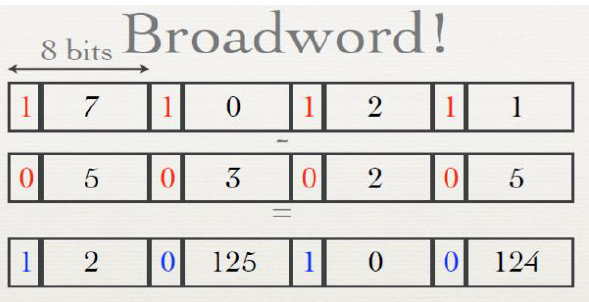
\includegraphics[width=100mm]{image/broad1.png}
	\label{fig:br1}
\end{figure}

Abbiamo due vettori di registri che sarebbero la mia bolla e la bolla del vicino. Voglio calcolare il massimo (7-3-2-5). Oltre il valore del vettore abbiamo un bit di supporto che rende più semplice capire il concetto, lo metto sopra a 1 e sotto a 0.
\bigbreak
Si fa una sottrazione: il prestito si propaga nei bit di supporto. Avremo 1 se non c'è stato bisogno di prestito, questo avviene se il minuendo era minore o uguale del sottraendo (nella prima colonna 7$>$5). Avremo 0 se il minuendo era piccolo rispetto al sottraendo e ha dovuto chiedere un prestito al bit di supporto (nella seconda colonna 0$<$3 per cui viene preso in prestito un bit e diventa $2^7 = 128 - 3 = 125$). 
\textbf{Se il bit di supporto è a 1 prendo quello sopra, se il bit di supporto va a 0 considero quello sotto}
\bigbreak
\noindent Questa è l'idea ora devo costruire una maschera che mi ridia i valori che mi servono.
\clearpage

\begin{figure}[h]
	\centering
	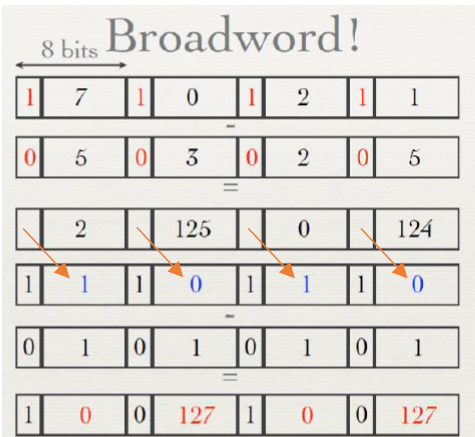
\includegraphics[width=100mm]{image/broad2.png}
	\label{fig:br2}
\end{figure}

I bit in blu sono la trascrizione dei bit di prestito ottenuti dalla sottrazione sopra (1 - 0 - 1 - 0), setto tutti i bit di supporto a 1. Successivamente sottraggo quello che ho ottenuto con una maschera fissa (bit di supporto = 0 e tutti i sottraendi a 1). 

In questo modo ottengo un vettore maschera o di tutti 0 o di tutti 1. Se ho tutti 0 devo prendere il valore della prima riga (7 - 2), se ho tutti 1 devo prendere il valore della seconda riga (3 - 5). 
\bigbreak
Faccio: maschera AND la seconda riga OR NOT (maschera) AND quello sopra

\chapter{Strutture dati succinte}
\label{cap:strutturedatisuccinte}
Uno struttura dati succinta utilizza uno schema di memorizzazione tale che lo spazio occupato sia al più ITLB e ciononostante è possibile effettuare operazioni tipiche. Un esempio è dato dagli alberi binari che vengono rappresentati in $log(4^n) = 2n$
\bigbreak
Non si tratta di compressione, la compressione si basa sulla predizione, cioè data una distribuzione dei dati si cerca di tarare una struttura dati per memorizzare con pochi bit i dati più frequenti. Succinto significa utilizzare il minimo spazio possibile che va bene per tutti gli input a prescindere dalla distribuzione. 

Nel nostro caso vogliamo memorizzare un insieme d n elementi, sottoinsieme di un insieme universo U. Sappiamo che ci sono $\binom{|U|}{|N|}$ sottoinsieme di N elementi, quindi dovremmo riuscire a utilizzare $log(\binom{|U|}{|N|)}$ bit, se n è abbastanza piccolo dovremmo riuscire a memorizzare in nlog(u/n). E' ITLB.

\section{Elias Fano}
\label{eliasfano} 
E' una struttura dati con degli operatori che in tempo costante permettono di:
\begin{itemize}
    \item recuperare i-esimo elemento
    \item trovare il primo elemento maggiore di un elemento dato (notiamo che un vettore esplicito non ci permette di farlo dovremmo fare una ricerca dicotomica).
\end{itemize}

Elia e Fano nel 1975 proposero una struttura dati quasi succinta (è buono quasi ITLB) per rappresentare sequenze monotone di numeri: si parla di strutture dati statiche, in cui se si cambia l'insieme di elementi si deve ricostruire l'intera struttura, ottimo per i motori ricerca che cambiano lentamente.
\bigbreak
L'idea è quella di utilizzare high bits/low bits. In una sequenza monotona crescente (cioè ci possono essere duplicati) possiamo distinguere segnali (bit alti) e rumore (bit bassi). Il segnale, essendo prevedibile, può essere memorizzato meglio, il rumore dev'essere memorizzato così com'è. 
\bigbreak
Consideriamo \textit{n} (numero di DocIDs, sequenza di n numeri) e \textit{u} (massimo valore dell'ID dei documenti), abbiamo la sequenza monotona crescente di numeri naturali $0 < x\textsubscript{0} < x\textsubscript{1} < ... < n\textsubscript{n-1} <= u$, con u upper bound sull'ultimo valore. Ciascun valore nella sequenza è rappresentato in binario, è poi diviso in due: $log(n)$ bit alti e $log(u)-log(n)$ bit bassi (anche scrivibile come $log(u/n)$).
\bigbreak
In figura consideriamo la lista 5,8,8,15,32 con upper bound = 36, per questo $l = log(36/5) = 2$
Prendiamo gli \textit{l = 2} bit bassi (esplicitamente senza compressione) e li concateniamo a formare il vettore dei bit bassi (vettore a dx in figura). A sinistra, i gap dei valori dei bit alti sono memorizzati sequenzialmente usando l'unario. 

\begin{figure}[h]
	\centering
	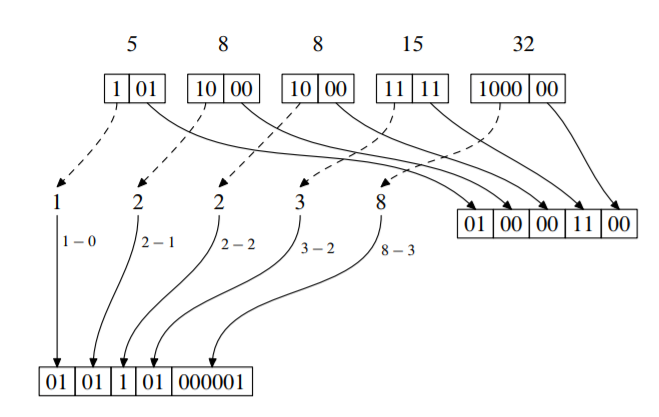
\includegraphics[width=120mm]{image/eliasfano1.png}
	\label{fig:ef1}
	\caption{}
\end{figure}

\bigbreak
La concatenazione dei bit bassi prende chiaramente \textit{nlog(u/n)} e la parte alta in unario occupa 
Usiamo al più 2+log(u/n) bit per elemento, l'ottimo sarebbe log(u/n). L'ultimo, log(u/n) è il costo inevitabile dato dai bit bassi. 1 = costo nel bit a 1 nel codice unario, 1 = è dato dal costo degli zeri dell’unario, ovvero, nell’array che memorizza i bit alti se aggiungiamo uno zero nei bit alti stiamo aumentando l’ordine del numero di 2l= u/n. Possiamo aggiungere al più n 0 prima di sforare il tetto di u, quindi è di fatto impossibile che ci siano più di n bit a 0 nell’array, quindi uno per elemento. 

Perché è fantastico Elias-Fano? Lo spazio occupato è quasi ottimo, è distribution free, leggere sequenzialmente richiede poche operazioni logiche (un clock per leggere un elemento dell’unario).  Tutte le operazioni di ricerca vengono fatte sui bit alti, quindi sono estremamente rapide:
Selezione del k-esimo elemento nella lista: si fa pop count fino ad arrivare al k-esimo 1. 
Ricerca primo elemento $>$ x:  faccio x/l = t. t è il numero di zeri che devono essere saltati prima di trovare il numero $>$ x, salto quei 5 e se ce ne sono altri salto ance quelli finché non trovo un uno. 

Altre proprietà utili: 
Il vettore dei gap scritti in unario ha una proprietà fondamentale: il rango + il valore dei bit alti è uguale alla posizione. 
Esempio: 01,01,1,01,000001
1 è in posizione 6, rango 3 – ovvero il numero di uno che lo precedono, 01 vale 1. 
3(rango) + 1(valore bit)  = 6(posizione)
Basta sapere 2 di questi valori per ricavare il terzo. In una tabella fissiamo dei quanti q e per ogni quanto memorizziamo la posizione del q-esimo 0/1 dei bit alti ed il rango, quindi riusciamo a ricavare il valore.

\chapter{Dimensionality reduction}
\label{dimensionalityreduction}
La relazione tra due entità può essere rappresentata comodamente da una matrice M: come esempio, la matrice termine/documento ha i termini come righe e i documenti come colonne. Ogni elemento nonnullo della matrice  (penso di aver capito che può contenere anche uno score assegnato a quel documento, tipo BM25) indica che il termine della riga appare nel documento in colonna. Per varie ragioni queste matrice sono molto sparse (in particolare i vettori rappresentanti i documenti).

Un'idea simile è un \textit{click matrix}, una matrice che ha come righe le query e gli URL come colonne. Questa matrice ha elemeno nonnullo quando un qualche utente ha cliccato la colonna URL per la query nella riga. 

In generale la "dimensionality reduction" consiste nel cambiare la rappresentazione delle entità usando un spazio di minore dimensione, usando vettori densi. 
\bigbreak
\noindent Possiamo scrivere la fattorizzazione della matrice M
\begin{equation}
    M = U \Sigma V^t
\end{equation}
chiamata \textbf{decomposizione in valori singolari}.
Nella formula U è una matrice ortogonale (trasposta = inversa) \textit{m}x\textit{m}, $\Sigma$ è una matrice \textit{m}x\textit{n} con gli unici elementi nonzero lungo la diagonale, e V è una matrice ortogonale \textit{n}x\textit{n}.
Gli elementi di $\Sigma$ sono detti \textit{valori singolari} di M. Il teorema di decomposizione ci dice che questa fattorizzazione è sempre possibile.
\bigbreak
Una matrice M \textit{m}x\textit{n} qualunque è una trasformazione lineare da uno spazio di dimensione n in uno di dimensione m, il teorema dice che qualsiasi trasformazione lineare può essere descritta da:
\begin{itemize}
    \item una rotazione n-dimensionale ($V^t$)
    \item moltiplicazione delle coordinate di ogni vettore per una costante (l'effetto di $\Sigma$ - espansione lineare lungo gli assi cartesiani)
    \item una rotazione m-dimensionale (l'effetto di U)
\end{itemize}
La decomposizione in valori singolari è un metodo classico di calcolare una riduzione di rango.

\section{Indicizzazione semantica latente}
\label{indlatente}
L'indicizzazione della semantica latente è una tecnica molto sofisticata basata sulla riduzione di rango. Intuitivamente l'idea è di vedere la matrice termini/documenti come una trasformazione lineare e ridurla di rango. La riduzione di rango dovrebbero portare ad una diminuzione del rumore (cioè dell'informazione non essenziale) della matrice termini/documenti, e faccia emergere una semantica latente, basata sulla coocorrenza dei termini.
\bigbreak
Facciamo un esempio, abbiamo tre documenti così fatti: "io parlo di cani", "cani e gatti", "io parlo di gatti". La matrice termini/documenti è quindi:

\begin{figure}[h]
	\centering
	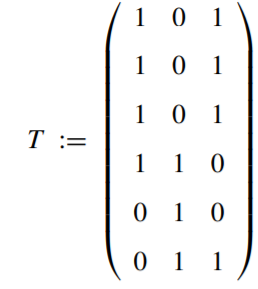
\includegraphics[width=40mm]{image/semantica1.png}
	\label{fig:ef1}
\end{figure}
Dove i termini sono enumerati in ordine di apparizione. La decomposizione a valori singolari ci da: 

\begin{figure}[h]
	\centering
	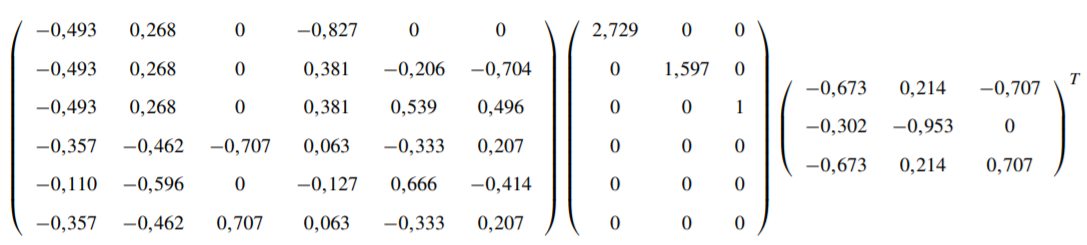
\includegraphics[width=130mm]{image/semantica2.png}
	\label{fig:ef1}
\end{figure}
Se ora operiamo un riduzione di rango eliminando il valore singolare più piccolo e rimoltiplichiamo, otteniamo:

\begin{figure}[h]
	\centering
	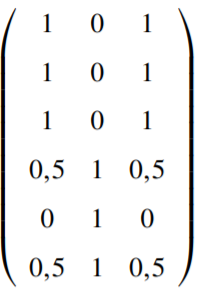
\includegraphics[width=40mm]{image/semantica3.png}
	\label{fig:ef1}
\end{figure}

La riduzione di rango ha schiacciato due concetti simili: da "cani" e "gatti" siamo arrivati ad "animale"; sia il primo che il terzo documento parlando di animali. La ragione per cui "cani" e "gatti" sono stati accomunati è cooncorrono nello stesso documento. Il fenomeno importante da osservare è che ora una documento può avere un valore positivo rispetto a un termine anche se il termine non compare nel documento. 

L'ipotesi alla base del procedimento è che esista una \textit{struttura semantica latente} all'interno della collezione: esiste un insieme latente di concetti, e ogni termine è più o meno in relazione con un concetto. Inoltre, ogni documento anch'esso più o meno in relazione con un concetto. La risoluzione di un'interrogazione avviene prendendo in considerazione i documenti relativi a dei concetti: potrei prendere un documento relativo al concetto ma che non comprende per forza il termine cercato. 

\chapter{Compressione dei grafi}
\label{compressionedeigrafi}
Studiare i Web graph è spesso complicato data la loro grande dimensione. Sono state proposte molte tecniche per poter mantenere i web graph in memoria, mostrando l'intrinseca ridondanza del web. 

Un web graph relativo ad un set di URL, è grafo orientato che ha gli URL come nodi e con un arco da \textit{x} a \textit{y} se una pagina \textit{x} contiene un hyperlink alla pagine \textit{y}. Per procedere mostriamo alcune considerazioni empiriche sulla struttura degli hyperlink. Le caratteristiche dei link sono chiamate \textit{locality} e \textit{similarity}.
\begin{itemize}
    \item \textbf{Locality}: molti link in una pagina portano l'utente a pagine con lo stesso host ("home", "next" etc); se noi compariamo gli URL sorgente e destinazione di questi link osserviamo che hanno un prefisso in comune; detto in altro modo se ordiniamo lessicograficamente quegli URL, essi saranno vicini. 
    \item \textbf{Similarity}: pagine che compaiono molto vicine tra loro (nell'ordine lessicografico) tendono ad avere successori comuni, questo perché molti link sono gli stessi nello stesso cluster locale di pagine. 
    \item \textbf{Consecutivity}: è possibile osservare che molti link in una pagina sono consecutivi. Primo perchè la struttura gerarchica del sito si riflette sugli URL, link al livello più basso della pagina tendono ad essere adiacenti nell'ordine lessicografico. 
\end{itemize}

Nodi, URL, vicini saranno quindi simili e la differenza (gap) tra loro piccola.
Queste caratteristiche suggeriscono l'uso di tecniche come codici istantanei per la memorizzazione di sequenze di numeri crescenti con gap piccoli. 
\clearpage

\section{Naive rapresentation}
\label{Naive}
Poniamo di essere interessati nel rappresentare un gruppo da N URL; i nodi del grafo saranno numerati da 0 a N-1 rispettando l'ordine lessicografico degli URL. S(x) indica il set di successori di x. Ci piacerebbe rappresentare il grafo usando una lista di adiacenza: il grafo sarà memorizzato come sequenza di lista di adiacenza dei nodi 0,1,etc, ognuno preceduto dal suo outdegree per riuscire a distinguere i vari vicinati. 

\noindent \textit{Alessia: E' una rappresentazione lenta, usiamo 64 bit per ogni successore}
\begin{figure}[h]
	\centering
	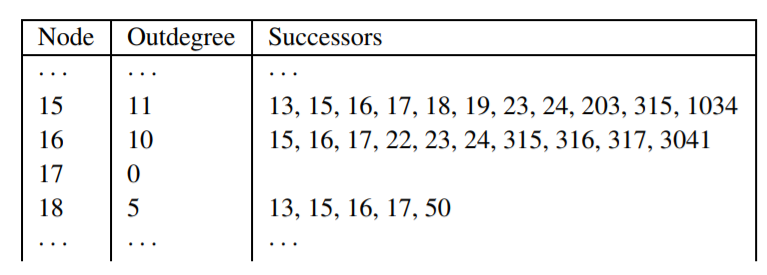
\includegraphics[width=110mm]{image/graphcomp2.png}
	\label{fig:ef1}
\end{figure}

\section{Using gaps}
\label{gaps}
La locality suggerisce che possiamo rappresentare ogni lista di successori come lista di gap. Più precisamente, se S(x) = (s1, ... , sk), la rappresenteremo invece in questo modo (s\textsubscript{1}-x,  s\textsubscript{2}-s\textsubscript{1}, s\textsubscript{3}-s\textsubscript{2}, .., s\textsubscript{k}-s\textsubscript{k-1}-1). Ogni intero ottenuto non è mai negativo, eccetto per il primo in qualche caso. Non volendo a avere a che fare con numeri negativi codifichiamo il primo elemento usando una funzione

\begin{figure}[h]
	\centering
	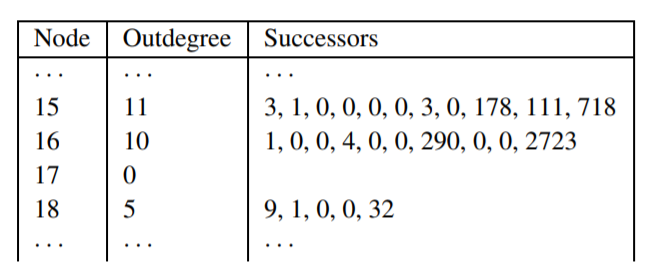
\includegraphics[width=110mm]{image/graphcomp1.png}
	\label{fig:ef1}
\end{figure}

\section{Reference compression}
\label{reference compression}
Dal momento che molte liste di successori sono simili, si può specificare la lista di successori di un nodo copiando parte della lista precedente, e aggiungere quello che manca (ad esempio usiamo una lista di bit, uno per ogni successore nella lista referenziata, che ci dica se il successore deve essere copiato o meno).
Chiamiamo S(y), la lista referenziata, x - y è il reference number (ogni nodo ne ha uno, indica a quale lista da copiare si riferisce) . Più precisamente la rappresentazione di S(x) rispetto a S(y) è formata da due parti: una sequenza di $|S(y)|$ bit, la lista copiata, e una lista di interi S(x)/S(y), la lista dei nodi extra. La copy list specifica quale dei link contenuti nella lista referenziata devo essere copiati: se e solo se contiene 1 alla i-esima posizione, l'elemento i-esimo della lista S(y) è copiata in S(x).

\begin{figure}[h]
	\centering
	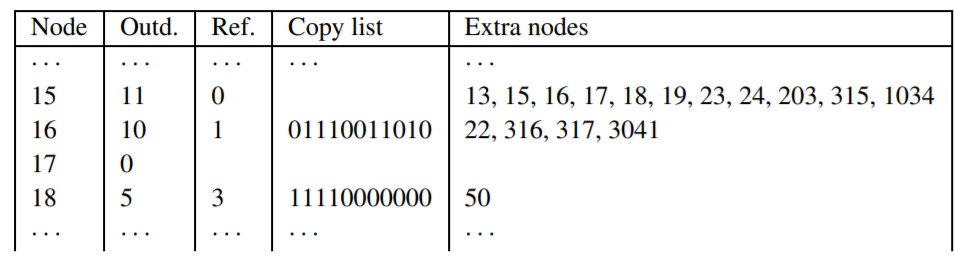
\includegraphics[width=120mm]{image/graphcomp3.png}
	\label{fig:ef1}
\end{figure}

\section{Offset array}
\label{offset}
Come abbiamo visto il grafo è descritto da una sequenza di liste di adiacenza; ogni lista è rappresentata da una sequenza crescente di numeri naturali, in ultimo luogo possiamo codificare questi interi con qualche codice (istantaneo penso). Se vogliamo accedere al grafo in modo random, abbiamo bisogno di un vettore ausiliario di offset, esso ha N elementi (uno per ogni nodo); l'elemento di indice \textit{h} rappresenta la posizione in memoria da dove parte la liste di successori del nodo h. 
La soluzione WebGraph implementata da Vigna e amichetti: se abbiamo bisogno di accessi random, ma abbiamo poco spazio in memoria possiamo caricare solo parzialmente l'array di offset. Più precisamente teniamo gli offset solo per i nodi 0, J, 2J con J parametro (jump). 
\clearpage
\section{Considerazioni generali fuori paper}
\label{considerazioni}

Abbiamo visto come tenere traccia dei successori, come gestiamo i predecessori? Dobbiamo memorizzare il grafo trasposto: il costo per ogni link è raddoppiato, avendo due rappresentazioni in memoria. L'adiacenza di due liste è lenta: prendo la lista di x, prendo la lista di y prendo la più corta e cerco se c'è l'altro elemento: lineare nel grado. 
\bigbreak
\noindent Le liste di successori sono liste di numeri crescenti, possiamo usare Elias Fano: comprime leggermente peggio un grafo ma abbiamo il vantaggio di poter vedere l'adiacenza in tempo costante. 
\bigbreak
\noindent Non stiamo rappresentando tutto il grafo in modo succinto, stiamo rappresentando ogni lista in modo succinto: siamo skillati nel comprimere le singole liste ma non è detto che lo siamo per tutto il grafo. 

\end{document}

